% =====================================================================
%  FINAL PAPER — IEEE conference, two column
%  A secure gateway-free LoRa mesh on ESP32
%
%  Build:  pdflatex final_paper && bibtex final_paper
%          && pdflatex final_paper && pdflatex final_paper
%
%  RESULTS AND CONCLUSION ARE DELIBERATELY EMPTY. Hardware testing has
%  not been done. Do not fill them with simulation output presented as
%  measurement — say which is which.
% =====================================================================
\documentclass[conference]{IEEEtran}
\IEEEoverridecommandlockouts

\usepackage{cite}
\usepackage{amsmath,amssymb}
\usepackage{graphicx}
\usepackage{booktabs}
\usepackage{array}
\usepackage{url}
\usepackage{tikz}
\usetikzlibrary{shapes.geometric, arrows.meta, positioning, calc, fit, backgrounds}

\begin{document}

\title{A Gateway-Free LoRa Mesh with End-to-End\\Authenticated Encryption on ESP32}

\author{
\IEEEauthorblockN{R.~Rakshith, S.~P.~Hegde, S.~G.~Uppalli, K.~S.~Suchit}
\IEEEauthorblockA{Department of Information Science and Engineering\\
B.M.S. College of Engineering, Bengaluru, India}
}

\maketitle

\begin{abstract}
Long-range radio is most useful where infrastructure is absent, but the protocol
normally layered on LoRa assumes a gateway with a backhaul. This paper describes
a messaging system that removes that assumption. Nodes built from an ESP32-S3 and
an SX1262 transceiver form a mesh in which every node originates, relays and
receives, and a phone attaches to any node over Bluetooth Low Energy to act as
the user interface. Routing uses a destination-sequenced distance-vector protocol
carried on the same beacon that performs neighbour discovery, so routing costs no
transmissions of its own, and the beacon interval scales with the number of nodes
a device knows about in order to hold aggregate control traffic roughly constant
as the mesh grows. Messages are encrypted with AES-128-GCM under a key agreed by
X25519 between the two endpoints and mixed with a pre-shared network key, which
means a relay cannot read what it forwards even though it holds the network key.
Separating the addresses a relay rewrites from the addresses the destination
authenticates is what makes that possible across multiple hops. We also describe
a link-layer authentication tag applied to every frame, a replay window tolerant
of the out-of-order delivery multi-hop routing produces, and a store-and-forward
mechanism that holds a message when its recipient is unreachable rather than
discarding it. Hardware evaluation is not complete; the experimental method is
given in Section~\ref{sec:setup} and results are deferred.
\end{abstract}

\begin{IEEEkeywords}
LoRa, mesh networking, ESP32, AES-GCM, X25519, DSDV, LPWAN security
\end{IEEEkeywords}

% =====================================================================
\section{Introduction}
% =====================================================================

The usual way to build a LoRa network is LoRaWAN, which puts gateways at the
centre and routes everything through a network server. It works well for sensors
reporting upward. It works badly when there is no gateway, and the situations
people cite to justify long-range radio — earthquakes, floods, mines, remote
fieldwork — are exactly the situations where there is no gateway, or where the
one that existed has just stopped working.

A mesh removes the dependency. If every node can relay, coverage grows with the
number of nodes rather than with the number of installed base stations, and two
people can exchange messages with nothing between them but other people's
radios. The routing problem this creates has been studied and has workable
answers on hardware costing very little~\cite{sole2022loramesher,
centelles2024dsdv, arregui2025gatewayfree}.

The security problem has not been answered in the same setting. LoRa frames are
easy to capture; Aras et al. demonstrated interception and bit-flipping with
inexpensive software-defined radio at ranges beyond the intended
link~\cite{aras2017exploring}. LoRaWAN's response is a pair of session keys, but
both are provisioned by the infrastructure that a gateway-free network does not
have. Meanwhile the mesh implementations that route well leave encryption out of
scope, and say so.

This paper describes a system that runs both at once on the same nodes. The
contributions are:

a packet format that lets a relay rewrite the fields it must while leaving the
payload and the end-to-end header cryptographically sealed; a key agreement
scheme that works without a server, in which the message key depends on both an
elliptic-curve exchange and a pre-shared network key so that breaking either
alone is not enough; a beacon that carries neighbour discovery, the distance
vector, the node's public key and its battery state in one frame, with an
interval that scales with mesh size; and an implementation with instrumentation
built in, so the quantities the design is supposed to satisfy can actually be
measured rather than asserted.

We are explicit about what is not here. The system has not been run on radios.
Section~\ref{sec:setup} sets out the measurements we intend to take;
Section~\ref{sec:results} is deliberately empty.

% =====================================================================
\section{Related Work}
% =====================================================================

Augustin et al. characterised the LoRa physical layer and produced the numbers
later work relies on, including the relationship between spreading factor,
payload length and time on air~\cite{augustin2016lora}. That relationship
constrains everything above it: bytes added to a frame become milliseconds of
channel occupancy, and in duty-cycled bands milliseconds are a regulated
resource~\cite{semtech2013toa}.

Cotrim and Kleinschmidt survey multi-hop approaches over LoRa and sort them into
flooding, tree or cluster structures, and general routing~\cite{cotrim2020lorawan}.
Solé et al. implemented a proactive distance-vector library for ESP32 in which
nodes periodically broadcast their routing tables~\cite{sole2022loramesher}; routes
are always ready, at the cost of control traffic that grows with the network.
Centelles et al. reduced that cost with a compact DSDV variant riding on
beacons~\cite{centelles2024dsdv}, following Perkins and Bhagwat's original
sequence-number mechanism~\cite{perkins1994dsdv}. Arregui Almeida et al. report a
gateway-free mesh on ESP32-S3 that chooses next hops reactively from signal
strength and recency, listens before transmitting, and recovers from node loss by
re-routing~\cite{arregui2025gatewayfree}. Our routing borrows from the last two and
our link layer from the third; none of the three encrypts anything.

On the security side, GCM is the standard choice for authenticated encryption on
a 32-bit microcontroller with an AES accelerator, and its specification is
unambiguous that a nonce must never repeat under one key~\cite{dworkin2007gcm}.
X25519 gives two nodes a shared secret with no server involved~\cite{rfc7748}, and
HKDF turns one secret into several keys bound to distinct
purposes~\cite{rfc5869}. For devices too small for AES, NIST selected ASCON as its
lightweight standard~\cite{nist2023ascon}. Formal analysis of LoRaWAN's own key
handling has found weaknesses in the join procedure~\cite{eldefrawy2019formal},
which is relevant here mainly as evidence that key establishment is where these
systems tend to break.

% =====================================================================
\section{System Architecture}\label{sec:arch}
% =====================================================================

A node is an ESP32-S3 with an SX1262 transceiver on the same board, an antenna
and a battery. A small display carries local diagnostics; the user interface
for messaging is a phone, attached over
Bluetooth Low Energy using the Nordic UART service, which is a de-facto profile
that behaves like a serial port and needs no pairing ceremony. The phone runs a
web application that can be installed to the home screen and cached, so after one
install it works with no network of any kind — which is the point, given where
these nodes are meant to go.

Figure~\ref{fig:arch} shows the arrangement. The node is a radio and a router;
the phone is the screen and the keyboard.

% ---------------------------------------------------------------------
%  DIAGRAM STUB — system architecture
%  Replace the layer names with your final module names if they change.
% ---------------------------------------------------------------------
\begin{figure}[!t]
\centering
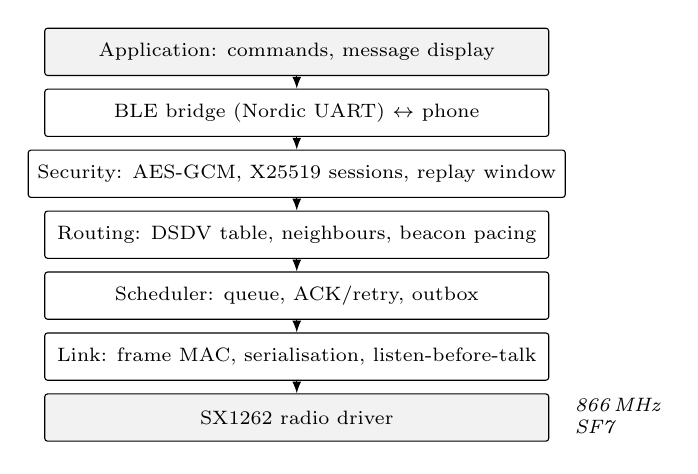
\begin{tikzpicture}[
  font=\scriptsize,
  lay/.style={draw, rectangle, minimum width=6.4cm, minimum height=6mm,
              align=center, rounded corners=1pt},
  arr/.style={-{Latex[length=1.5mm]}}
]
\node[lay, fill=black!5] (app)  {Application: commands, message display};
\node[lay, below=1.6mm of app]  (ble)  {BLE bridge (Nordic UART) $\leftrightarrow$ phone};
\node[lay, below=1.6mm of ble]  (sec)  {Security: AES-GCM, X25519 sessions, replay window};
\node[lay, below=1.6mm of sec]  (rt)   {Routing: DSDV table, neighbours, beacon pacing};
\node[lay, below=1.6mm of rt]   (sch)  {Scheduler: queue, ACK/retry, outbox};
\node[lay, below=1.6mm of sch]  (link) {Link: frame MAC, serialisation, listen-before-talk};
\node[lay, below=1.6mm of link, fill=black!5] (phy) {SX1262 radio driver};

\foreach \a/\b in {app/ble, ble/sec, sec/rt, rt/sch, sch/link, link/phy}
  \draw[arr] (\a) -- (\b);

\node[right=2mm of phy, font=\scriptsize\itshape, align=left] {866\,MHz\\SF7};
\end{tikzpicture}
\caption{Node software stack. Each layer is a separate module; the phone attaches
at the top, the radio at the bottom.}
\label{fig:arch}
\end{figure}

The firmware is organised as separate modules for the radio driver, packet
serialisation, security primitives, session keys, routing, scheduling, the link
layer and the BLE bridge. They compile as a single translation unit, which is an
inheritance from the Arduino build model rather than a design choice, and it
means module boundaries are enforced by discipline rather than by the linker.

% =====================================================================
\section{Protocol Design}\label{sec:protocol}
% =====================================================================

\subsection{Frame types}

Seven frame types share one channel. \textsc{data} carries a user message.
\textsc{ack} confirms one hop. \textsc{hello} is the beacon. \textsc{alt} tells a
sender that a next hop has already seen a packet and that another route should be
tried. \textsc{key\_req} and \textsc{key\_resp} fetch a public key from a node
more than one hop away. \textsc{receipt} tells the original sender that a message
actually arrived. Broadcast alerts reuse the \textsc{data} structure with a
reserved destination address.

\subsection{Packet format}

The \textsc{data} header is the part of the design that everything else depends
on, so it is worth being precise about. It carries two distinct address pairs.
The source and destination identify the endpoints and never change. The previous
and next hop identify the current radio link and are rewritten by every relay.
The time-to-live is decremented at each hop.

Only the first pair, together with the message identifier, sequence number and
payload length, is covered by the authenticated-associated-data input to the
cipher. The hop fields and the time-to-live are deliberately outside it, because
a relay has to change them. Figure~\ref{fig:frame} shows the layout.

% ---------------------------------------------------------------------
%  DIAGRAM STUB — DATA frame layout
% ---------------------------------------------------------------------
\begin{figure}[!t]
\centering
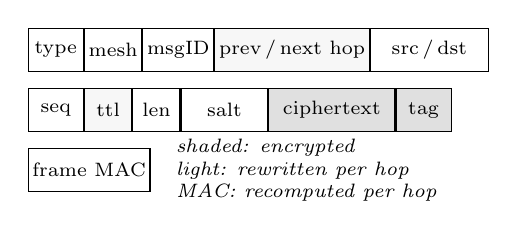
\begin{tikzpicture}[font=\scriptsize, node distance=0mm]
\tikzstyle{f}=[draw, minimum height=5.5mm, align=center, inner sep=1.5pt]
\tikzstyle{sealed}=[f, fill=black!12]
\tikzstyle{open}=[f, fill=white]

\node[open, minimum width=0.7cm] (t)  {type};
\node[open, minimum width=0.7cm, right=of t]  (m)  {mesh};
\node[open, minimum width=0.9cm, right=of m]  (id) {msgID};
\node[open, minimum width=1.5cm, right=of id, fill=black!3] (hop) {prev\,/\,next hop};
\node[open, minimum width=1.5cm, right=of hop] (e)  {src\,/\,dst};

\node[open, minimum width=0.7cm, below=2mm of t.south west, anchor=north west] (s) {seq};
\node[open, minimum width=0.6cm, right=of s, fill=black!3] (ttl) {ttl};
\node[open, minimum width=0.6cm, right=of ttl] (len) {len};
\node[open, minimum width=1.1cm, right=of len] (salt) {salt};
\node[sealed, minimum width=1.6cm, right=of salt] (ct) {ciphertext};
\node[sealed, minimum width=0.7cm, right=of ct] (tag) {tag};

\node[open, minimum width=1.2cm, below=2mm of s.south west, anchor=north west] (mac) {frame MAC};

\node[right=2mm of mac, align=left, font=\scriptsize\itshape]
  {shaded: encrypted\\light: rewritten per hop\\MAC: recomputed per hop};
\end{tikzpicture}
\caption{\textsc{data} frame. The endpoint addresses are authenticated; the hop
addresses and TTL are not, because relays must change them. The frame MAC covers
everything and is recomputed at each hop.}
\label{fig:frame}
\end{figure}

A message of the maximum length produces a frame that fits inside a single LoRa
transmission, so there is no fragmentation and no reassembly anywhere in the
system. That was a deliberate sizing decision: reassembly across a lossy
multi-hop path is a large amount of machinery to get wrong.

\subsection{Routing}

Routing is destination-sequenced distance vector. Each node owns a sequence
number that only it increments, in steps of two so the value is always even. A
node that detects a broken link advertises that destination's sequence plus one —
an odd number — with an infinite metric. Because a route is preferred when it is
fresher, or equally fresh and shorter, the odd invalidation outranks the stale
reachable routes neighbours still hold, and cannot be undone until the
destination itself issues a fresh even number. This is Perkins and Bhagwat's
mechanism~\cite{perkins1994dsdv} and it is what stops the count-to-infinity
behaviour a plain distance-vector protocol shows when a link fails.

The distance vector rides on the beacon rather than in its own messages. A beacon
therefore carries neighbour discovery, the routing table, the node's public key,
its name and its battery voltage together. This matters more than it sounds: on a
link this slow, a separate routing protocol would compete with user traffic for
the same duty-cycle budget.

Beacon pacing is adaptive. Interval is the number of nodes the device knows about
multiplied by the airtime of its own beacon and a constant, clamped to a range.
The reasoning is that $N$ nodes beaconing every $T$ seconds put $N \times
\mathit{airtime} / T$ of permanent load on one shared channel; holding that
product roughly constant keeps the control load from growing with the network.
A node that detects a broken link beacons early rather than waiting out the
interval, so invalidations propagate ahead of the timer. Good news is left to the
next scheduled beacon, which avoids a storm when a mesh powers up.

Figure~\ref{fig:route} traces a message.

% ---------------------------------------------------------------------
%  DIAGRAM STUB — routing and delivery flow
% ---------------------------------------------------------------------
\begin{figure}[!t]
\centering
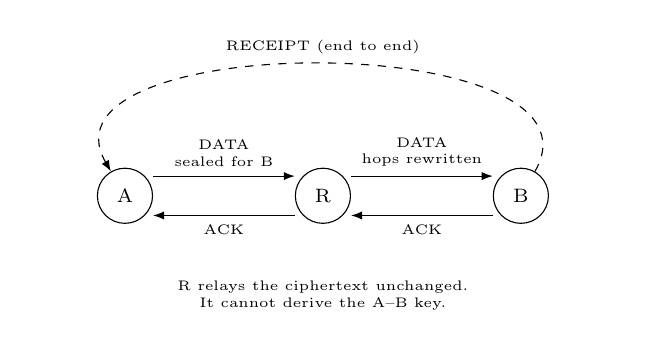
\begin{tikzpicture}[
  font=\scriptsize,
  n/.style={draw, circle, minimum size=7mm},
  arr/.style={-{Latex[length=1.4mm]}},
  lbl/.style={font=\tiny, align=center}
]
\node[n] (a) {A};
\node[n, right=1.8cm of a] (r) {R};
\node[n, right=1.8cm of r] (b) {B};

\draw[arr] ([yshift=2.5mm]a.east) -- node[lbl, above] {DATA\\sealed for B} ([yshift=2.5mm]r.west);
\draw[arr] ([yshift=-2.5mm]r.west) -- node[lbl, below] {ACK} ([yshift=-2.5mm]a.east);
\draw[arr] ([yshift=2.5mm]r.east) -- node[lbl, above] {DATA\\hops rewritten} ([yshift=2.5mm]b.west);
\draw[arr] ([yshift=-2.5mm]b.west) -- node[lbl, below] {ACK} ([yshift=-2.5mm]r.east);

\draw[arr, dashed] (b) to[out=60, in=120] node[lbl, above] {RECEIPT (end to end)} (a);

\node[below=6mm of r, lbl, align=center]
  {R relays the ciphertext unchanged.\\It cannot derive the A--B key.};
\end{tikzpicture}
\caption{Delivery across one relay. Hop acknowledgments confirm each link; the
receipt is what tells A the message arrived.}
\label{fig:route}
\end{figure}

\subsection{Delivery and retries}

Each hop acknowledges. An unacknowledged packet is retried a fixed number of
times, then the sender tries an alternate next hop. If that is also exhausted the
message is not discarded: it is held, still encrypted, and re-sent when a route
to the destination reappears. Holding is bounded by both a time limit and an
attempt count, because each attempt costs a transmission and its retries, and an
unbounded retry against a node that never returns is an airtime problem rather
than a persistence feature.

A hop acknowledgment proves only that the next radio heard the frame. End-to-end
delivery is proved by a receipt returned by the destination, carrying a short
authentication tag computed under the pair's session key so that only the real
destination can produce one. Without that, any mesh member could fake a delivery
confirmation, and the delivery ratio we intend to measure would be meaningless.

Broadcast alerts flood rather than route. Spread is bounded by a time-to-live and
by the duplicate history, so a node acts on the first copy it sees and drops the
rest; each node therefore transmits a given alert at most once.

% =====================================================================
\section{Security Design}\label{sec:security}
% =====================================================================

\subsection{Threat model}

We assume an attacker with a LoRa radio in range who can listen, transmit, and
record for later. Interception is free and undetectable~\cite{aras2017exploring}.
We do not assume physical security of the nodes: one may be captured and read.

The system distinguishes members of the mesh from outsiders, and this is the
honest boundary of what it achieves. An outsider cannot read messages, cannot
inject routing updates, and cannot forge acknowledgments. A member — or an
attacker who extracts the network key from a captured node — can forge control
frames and broadcasts. What such an attacker still cannot do is read a one-to-one
message it merely relays, and that is the specific property the elliptic-curve
layer buys.

\subsection{Keys}

Three keys are derived from a pre-shared network key with HKDF-SHA256, each under
a different context label so that none can be used in another's
role~\cite{rfc5869}. One authenticates frames. One encrypts broadcasts. The third
is per-pair and is not derived from the network key alone.

Each node generates an X25519 keypair on first boot and keeps the private half in
non-volatile storage. The message key for a pair of nodes is
\[
K_{ab} = \mathrm{HKDF}\bigl(\mathit{salt},\;
  X25519(a_{\text{priv}}, b_{\text{pub}}) \,\|\, K_{\text{master}},\;
  \mathit{label} \,\|\, \mathit{lo} \,\|\, \mathit{hi}\bigr)
\]
where $\mathit{lo}$ and $\mathit{hi}$ are the two node identifiers in a fixed
order so both ends derive the same key. Mixing the elliptic-curve secret with the
pre-shared key means an attacker must break both mechanisms rather than either.
A relay holds $K_{\text{master}}$ like everyone else but neither private key, so
it cannot compute $K_{ab}$.

Public keys travel on the beacon, which means a session with any direct neighbour
costs no round trip. Nodes further away are fetched on demand when a message is
first addressed to them. An earlier design fetched keys for every destination in
the routing table as soon as it appeared; that is quadratic in the number of
nodes, and in simulation it dominated channel traffic to set up sessions that
were mostly never used.

Received public keys are checked before use. A point of small order produces a
fixed shared secret that the sender knows without holding any private key, so
such keys are rejected as RFC 7748 requires~\cite{rfc7748}.

\subsection{Message protection}

Payloads are encrypted with AES-128-GCM, which gives confidentiality and
integrity in one pass~\cite{dworkin2007gcm}. The tag is verified before any
plaintext is released. The authenticated-associated-data input covers the
endpoint addresses, message identifier, sequence number and payload length, so a
relay that alters any of them invalidates the tag.

GCM requires that a nonce never repeat under a given key, and the consequences of
repetition are severe rather than gradual: reuse exposes the exclusive-or of two
plaintexts and the authentication subkey~\cite{dworkin2007gcm}. Building a nonce
from counters is therefore only safe while every counter outlives the key. Ours
did not. The broadcast key is derived from a compiled-in network key and survives
a wipe of non-volatile storage, while the sequence number and message counter
that fed the nonce both restart. The first broadcast after such a wipe reused the
nonce of the first broadcast before it.

The fix is to stop depending on counters. Each message carries eight bytes drawn
from the hardware random generator when it is sealed, and the nonce is those
bytes followed by the sequence number. The salt is carried by relays unchanged,
because it is part of what was sealed; altering it changes the nonce and the tag
then fails, so it needs no separate protection.

\subsection{Replay}

Each node keeps a sliding window per source: the highest sequence number accepted
and a bitmap of recent ones, so that out-of-order arrival — which multi-hop
routing produces routinely — is tolerated while repeats are rejected. The window
is consulted only after the tag verifies. Checking an unauthenticated sequence
number first would let an attacker advance the window with forged values and lock
out the genuine sender.

Sequence numbers are reserved from non-volatile storage in blocks, so a reboot
resumes past the whole reserved block rather than replaying numbers, without
writing to flash on every message. When a new session key is agreed with a peer
the window for that peer is cleared, because replay protection has meaning only
inside a key epoch: an old message cannot decrypt under a new key, so retaining
the window protects nothing and would lock out a peer whose storage had been
erased.

\subsection{Frame authentication}

Every frame carries a truncated HMAC-SHA256 tag under the network control key,
and nothing is parsed until it verifies. This is what stops an outsider injecting
routing beacons — which, once routing became table-driven, would otherwise let
them claim a one-hop route to any node and attract its traffic. Tags are compared
without short-circuiting, so a failed comparison does not reveal how much of a
guess was correct. On \textsc{data} the frame tag sits underneath the end-to-end
GCM tag and is recomputed at each hop, since relays legitimately rewrite the hop
fields.

% =====================================================================
\section{Implementation}\label{sec:impl}
% =====================================================================

Firmware is C++ built with PlatformIO for the Arduino-ESP32 core. The radio is
driven through RadioLib, which supports both the SX1262 on the primary board and
the SX1276 variant behind the same interface. Cryptography uses mbedTLS as
shipped with the ESP-IDF, which provides AES-GCM with hardware acceleration and
Curve25519 arithmetic. HKDF is implemented over HMAC because the HKDF module is
not enabled in the stock configuration.

The radio is interrupt-driven only to the extent of setting a flag. Reading a
frame, and everything above that, happens in the main loop, so nothing touches
SPI from interrupt context. Before transmitting, a node performs channel activity
detection using the transceiver's own hardware, which answers in a few
milliseconds; an earlier design listened for a fixed window before every frame,
which on a three-hop path consumed most of the latency budget.

Table~\ref{tab:params} lists the operating parameters. Frequency is set for the
Indian 865--867\,MHz licence-exempt band.

\begin{table}[!t]
\caption{Operating parameters}
\label{tab:params}
\centering
\footnotesize
\begin{tabular}{@{}ll@{}}
\toprule
Parameter & Value \\
\midrule
Microcontroller & ESP32-S3 \\
Transceiver & SX1262 \\
Frequency & 866.0\,MHz \\
Spreading factor / bandwidth & SF7 / 125\,kHz \\
Coding rate & 4/5 \\
Transmit power & 14\,dBm \\
Maximum message length & 200 characters \\
Cipher & AES-128-GCM \\
Key agreement & X25519 \\
Key derivation & HKDF-SHA256 \\
\bottomrule
\end{tabular}
\end{table}

The phone application is a web page using Web Bluetooth, installable so that it
runs from cache with no network. It shows conversations, the node list with
signal and encryption state, delivery status, and a diagnostics pane exposing
every firmware command. Position sharing uses the phone's own receiver rather
than a module on the node, and travels as an ordinary encrypted message with a
recognised prefix, so it needs no firmware support.

One limitation of that choice is worth stating: Web Bluetooth is unavailable on
iOS in any browser, because every iOS browser is required to use the same
underlying engine. iPhone users need a third-party browser that bridges
Bluetooth natively, or a native application would have to be written.

% =====================================================================
\section{Experimental Setup}\label{sec:setup}
% =====================================================================

Evaluation has two halves, and we keep them separate because they prove different
things.

\subsection{Simulation}

A discrete-time simulator models the protocol with a shared channel, computing
time on air from the standard LoRa equation~\cite{semtech2013toa} and treating
any overlap at a receiver as a lost frame, which is pessimistic because it
ignores the capture effect. It reimplements the routing, key discovery,
acknowledgment, flooding and store-and-forward logic from the firmware headers.
It does not execute the firmware, so it cannot find defects in that code; what it
can test is whether the protocol behaves at a scale we cannot build.

Planned runs cover 3, 10 and 20 nodes, each with a node-failure and rejoin
scenario and a partition in which the field is split and later rejoined.
Recorded quantities are convergence time, end-to-end delivery ratio, latency,
peak table occupancy against the configured limits, per-node duty cycle and
collision rate.

\subsection{Hardware}

Five nodes. Three arrangements: all within range of each other; a line forcing
two and three hops; and a layout with two disjoint paths between endpoints so
that an intermediate node can be removed without partitioning the mesh.

Measurements come from instrumentation already in the firmware, read over the
phone or the serial console. The firmware records messages sent, first-hop
acknowledgments, end-to-end receipts, retransmissions, relayed and duplicate
frames, security events, per-operation encryption and decryption time in
microseconds, and accumulated airtime from which duty cycle is computed.

Delivery ratio is receipts against messages sent, measured at the sender.
First-hop acknowledgment ratio is recorded alongside it, because the gap between
the two localises loss beyond the first link. Latency is measured on one node's
own clock from queueing to acknowledgment, which avoids needing synchronised
clocks across the mesh; this understates full end-to-end time on a multi-hop
path and we will report it as what it is.

Planned trials: delivery and latency against hop count; behaviour when a relay is
switched off mid-conversation and brought back; broadcast coverage; and time from
power-on to a converged routing table.

% =====================================================================
\section{Results}\label{sec:results}
% =====================================================================

% =====================================================================
%  PLACEHOLDER — NOTHING HERE YET
%
%  Hardware trials have not been run. Do not populate this section with
%  simulation output written as though it were measurement. If you
%  report simulation figures, put them in their own subsection and label
%  them as simulation in the text, the table caption and the figure
%  caption.
%
%  Suggested structure once data exists:
%    A. Simulated behaviour at 3, 10 and 20 nodes
%    B. Delivery ratio and latency by hop count (hardware)
%    C. Recovery from node loss and rejoin
%    D. Cryptographic cost per message, measured
%    E. Duty cycle and airtime against the regulatory budget
% =====================================================================

\textit{[Placeholder. Hardware evaluation has not been carried out. This section
will report measured results once the trials in Section~\ref{sec:setup} have been
run. Simulation figures, where reported, will be labelled as simulation.]}

% =====================================================================
\section{Conclusion}
% =====================================================================

% =====================================================================
%  PLACEHOLDER — write this after the results exist.
%  A conclusion that does not depend on your own measurements is not a
%  conclusion, it is an abstract with a different heading.
% =====================================================================

\textit{[Placeholder. To be written once results are available.]}

\bibliographystyle{IEEEtran}
\bibliography{references}

\end{document}
